\documentclass[11pt]{article}
\usepackage[letterpaper,margin=0.72in]{geometry}
\usepackage{amsmath,amssymb,amsthm,mathtools}
\usepackage{graphicx}
\usepackage[T1]{fontenc}
\usepackage{microtype}
\setlength{\parindent}{0pt}
\setlength{\parskip}{0.38em}
\setlength{\emergencystretch}{2em}
\newtheorem{theorem}{Theorem}
\newtheorem{lemma}{Lemma}
\newcommand{\Op}{\operatorname{Op}}
\newcommand{\Ell}{\operatorname{Ell}}
\newcommand{\cB}{\mathcal B}
\newcommand{\cT}{\mathcal T}
\newcommand{\specop}{\operatorname{spec}}
\title{Continuity of the sectorial bounded holomorphic calculus\\
\large A full answer to the open problem in arXiv:1101.0067}
\author{Run \texttt{fa\_banach\_001} --- \texttt{agent\_lane\_03}}
\date{12 August 2026}

\begin{document}
\maketitle

\textbf{Status.} High-confidence candidate full proof, pending human review.
The only normalization needed is made explicit below: since the source gives
$f$ only on the selected sector, $f(A)$ means $f$ on that spectral sector and
zero on the other one.  For $f\equiv1$ this is exactly the source's sectorial
projection.

\section*{The source question}
Let $M$ be closed, $E\to M$ Hermitian, $m>0$, and let $\Gamma_+$ be the
fixed two-ray contour of the source.  It divides the plane into sectors
$\Lambda_+$ and $\Lambda_-$.  The source proves continuity of
$A\mapsto P_{\Gamma_+}(A)$ on $\Ell^m_{\Gamma_+}(M,E)$ in its topology
$\cT$, and asks whether the theorem extends to bounded holomorphic functions.

\begin{center}
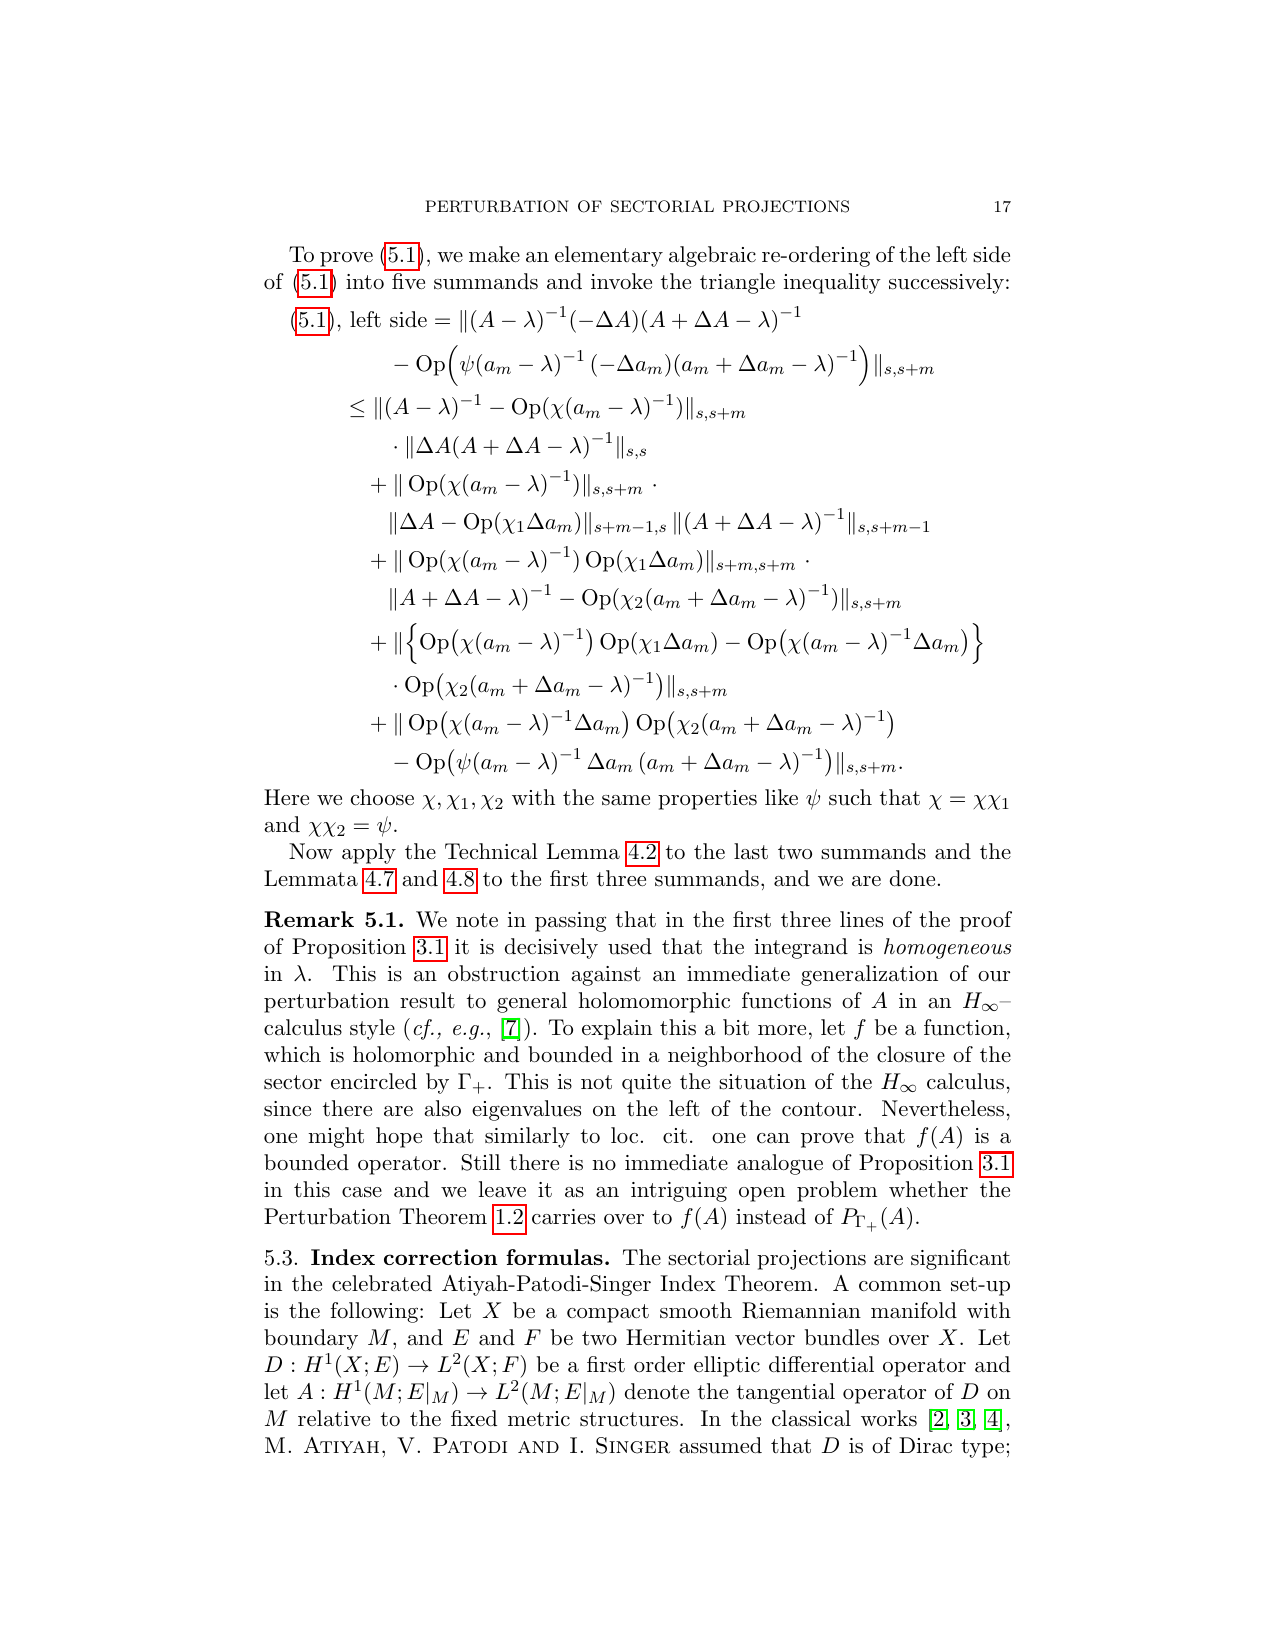
\includegraphics[width=0.90\textwidth,trim=45 195 45 430,clip]{figures/source_open_problem_page_17.png}
\end{center}

The exact page is bundled as \texttt{source\_excerpt\_open\_problem\_page\_17.pdf}.

Fix disjoint open neighborhoods $U_\pm$ of the closed sectors and
$f\in H^\infty(U_+)$.  Put
\[
 F(z)=\begin{cases}f(z),&z\in U_+,\\0,&z\in U_- .\end{cases}
\]
Thus $F$ is holomorphic on the disconnected neighborhood $U_+\cup U_-$.
Write $f_{\Gamma_+}(A):=F(A)$ for the corresponding sectorial holomorphic
calculus, initially for functions decaying at zero and infinity and then by
the standard bounded-calculus convergence procedure.

\begin{theorem}\label{thm:main}
For every $s\in\mathbb R$ and every fixed $f\in H^\infty(U_+)$, the operator
$f_{\Gamma_+}(A)$ is bounded on $H^s(M;E)$ and
\[
 \Ell^m_{\Gamma_+}(M,E)\longrightarrow\cB(H^s(M;E)),
 \qquad A\longmapsto f_{\Gamma_+}(A),
\]
is continuous in the source topology $\cT$.  Locally in $A$ one has
$\|f_{\Gamma_+}(A)\|_{s,s}\le C\|f\|_\infty$.
\end{theorem}

\section*{The two ingredients}
Write the topology exactly as the source does:
\[
 A=\Op(a_m)+B,\qquad
 a_m\in C^\infty(S^*M;\operatorname{End}(\pi^*E)),\qquad
 B\in\Psi^{m-1}(M;E).
\]
Then $A_j\to A$ in $\cT$ means $a_m(A_j)\to a_m(A)$ in $C^\infty$ and
\[
 \|B(A_j)-B(A)\|_{k+m-1,k}\longrightarrow0
 \quad\text{for every integer }k.                                      \tag{1}
\]
Interpolation gives the analogous statement at all real Sobolev indices.

The first ingredient is the symbol-level bounded holomorphic calculus of
Bilyj--Schrohe--Seiler.  Their Theorems 3.2 and 3.5 prove that bounded
holomorphic functions of a sectorially parameter-elliptic symbol are symbols
of order zero, with every symbol seminorm and the induced operator norm
bounded by $C\|f\|_\infty$.  Their proof uses local Cauchy contours around the
pointwise symbol spectrum.  Consequently it applies componentwise to $F$:
the contours around the $+$ component contribute $f$, while those around the
$-$ component contribute zero.

\begin{lemma}[frozen lower-order family]\label{lem:frozen}
Fix $A_0=\Op(a_0)+B_0$.  For $a$ in a sufficiently small $C^\infty$
neighborhood of $a_0$, set $C(a)=\Op(a)+B_0$.  Then
\[
 a\longmapsto f_{\Gamma_+}(C(a))\in\cB(H^s)
\]
is continuous and locally bounded by $C\|f\|_\infty$.
\end{lemma}

\emph{Justification.}
Uniform separation of the principal spectrum from the two cutting rays
persists in a $C^0$ neighborhood.  On the unbounded part, the cited
parameter-dependent construction gives an order-zero symbol; the resolvent
identity on its local Cauchy contours makes each symbol seminorm continuous
in $a$.  The finitely many bounded spectral points are enclosed by a compact
Dunford contour, where ordinary resolvent continuity applies.  Quantization
$\Psi^0\to\cB(H^s)$ is continuous.  This proves the lemma.  Notice that the
lower-order symbol is fixed, so no topology stronger than $\cT$ is being
silently imposed.

The second ingredient is the extra resolvent produced by comparing two
operators.  Put
\[
 \delta:=\min\{1,1/m\}.
\]

\begin{lemma}[integrable resolvent difference]\label{lem:two}
Let $A,C$ lie in a sufficiently small $\cT$-neighborhood, have the same
principal symbol, and put $D=A-C\in\Psi^{m-1}$.  On either unbounded ray of
$\Gamma_+$,
\[
 \|(A-\lambda)^{-1}D(C-\lambda)^{-1}\|_{s,s}
 \le C_s\,q_s(D)|\lambda|^{-1-\delta},                    \tag{2}
\]
where
\[
 q_s(D)=
 \begin{cases}
 \|D\|_{s+m-1,s},&m\ge1,\\
 \|D\|_{s,s+1-m},&0<m<1.
 \end{cases}
\]
Both are continuous seminorms of $\cT$.
\end{lemma}

\emph{Proof.}
The source's minimal-growth estimate is
\[
 \|(T-\lambda)^{-1}\|_{u,u+p}
 \le C|\lambda|^{-1+p/m},\qquad 0\le p\le m,              \tag{3}
\]
locally uniformly in $T$.  If $m\ge1$, apply (3) with $p=m-1$ to
the right resolvent, then $D:H^{s+m-1}\to H^s$, and apply (3) with
$p=0$ to the left resolvent.  This gives
$|\lambda|^{-1/m}|\lambda|^{-1}$.  If $0<m<1$, use both resolvents
on their fixed Sobolev spaces with decay $|\lambda|^{-1}$ and use the
smoothing map $D:H^s\to H^{s+1-m}$ between them.  This gives
$|\lambda|^{-2}$.  These are exactly (2). \qed

\section*{Proof of Theorem \ref{thm:main}}
Fix $A_0=\Op(a_0)+B_0$.  For nearby $A=\Op(a)+B$, freeze its lower-order
part at the base point:
\[
 C=C(a):=\Op(a)+B_0,\qquad D:=A-C=B-B_0.                  \tag{4}
\]
Then $C\to A_0$ in the ordinary full-symbol topology, while (1) says
$q_s(D)\to0$.

First take a holomorphic $f$ with the usual decay at zero and infinity.
The resolvent identity gives, with the standard orientation,
\[
 f_{\Gamma_+}(A)-f_{\Gamma_+}(C)
 =\frac1{2\pi i}\int_{\Gamma_+}
 f(\lambda)(A-\lambda)^{-1}D(C-\lambda)^{-1}\,d\lambda.  \tag{5}
\]
By Lemma \ref{lem:two}, the two rays contribute at most
\[
 C_s\|f\|_\infty q_s(D)
 \int_R^\infty r^{-1-\delta}\,dr.
\]
The connecting compact arc contributes the same type of bound by uniform
resolvent continuity.  Hence
\[
 \|f_{\Gamma_+}(A)-f_{\Gamma_+}(C)\|_{s,s}
 \le K_s\|f\|_\infty q_s(D).                              \tag{6}
\]

Choose the standard bounded holomorphic regularizers $\rho_n$, decaying at
zero and infinity, with uniformly bounded sup norms and $\rho_n\to1$ locally
uniformly on both sectors.  Estimate (6), uniform in $n$, and the bounded
calculus convergence lemma pass (5)--(6) from $\rho_nF$ to every bounded
$F$.  This proves boundedness of $f_{\Gamma_+}(A)$ and retains (6).

Finally,
\begin{align*}
 \|f_{\Gamma_+}(A)-f_{\Gamma_+}(A_0)\|_{s,s}
 &\le K_s\|f\|_\infty q_s(B-B_0)\\
 &\quad+\|f_{\Gamma_+}(C(a))-f_{\Gamma_+}(C(a_0))\|_{s,s}.
\end{align*}
The first term tends to zero by (1), and the second by Lemma
\ref{lem:frozen}.  This proves continuity at the arbitrary base point $A_0$.
The same estimates give the local norm bound. \qed

\section*{Proof intuition and scope}
The source's direct integral has only one resolvent and therefore decays like
$|\lambda|^{-1}$, exactly at the divergent endpoint.  Freezing the lower
order part separates the two pieces of $\cT$.  Principal-symbol variation is
handled by the established bounded symbol calculus; lower-order variation is
handled by a resolvent difference, which automatically contains two
resolvents.  The order gap of one supplies the additional
$|\lambda|^{-\delta}$ that makes the contour integral converge.

The result answers Remark 5.1 under the canonical sectorial interpretation.
It does not assert continuity when the function $f$ itself varies without a
uniform holomorphic domain, nor does it weaken the source's fixed-cut and
minimal-growth hypotheses.  Exact-ID, title, citation, and official-arXiv
searches through 12 August 2026 found no later paper explicitly closing this
perturbation question; this is a bounded novelty audit, not a priority claim.

\section*{References}
\begingroup\raggedright
\textbf{[1]} B. Boo\ss--Bavnbek, G. Chen, M. Lesch, and C. Zhu,
\emph{Perturbation of Sectorial Projections of Elliptic
Pseudo-differential Operators}, arXiv:1101.0067, Theorem 1.2,
Definition 2.7, Lemma 4.7, and Remark 5.1.

\textbf{[2]} O. Bilyj, E. Schrohe, and J. Seiler,
\emph{$H_\infty$-calculus for hypoelliptic pseudodifferential operators},
arXiv:0901.3160, Theorems 3.2 and 3.5.
\par\endgroup

\end{document}
